\documentclass[standalone, version=1.0]{huangfusl-template}
\usepackage{tikz}
\begin{document}
    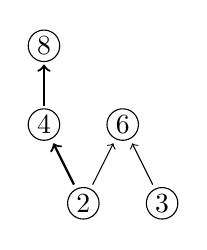
\begin{tikzpicture}
        \node (A) at (-0.5,0){$2$};
        \node (B) at (0.5,0){$3$};
        \node (C) at (-1,1){$4$};
        \node (D) at (0,1){$6$};
        \node (E) at (-1,2){$8$};
        \draw (A) circle (0.2);
        \draw (B) circle (0.2);
        \draw (C) circle (0.2);
        \draw (D) circle (0.2);
        \draw (E) circle (0.2);
        \draw[thick,-to] (A) -- (C);
        \draw[-to] (A) -- (D);
        \draw[-to] (B) -- (D);
        \draw[thick,-to] (C) -- (E);
    \end{tikzpicture}
\end{document}